\documentclass[a4paper,10pt]{article}
\usepackage[utf8]{inputenc}

%pour les equations
\usepackage{amsmath}
\usepackage{amssymb}
\usepackage{amsfonts}

%pour les images
\usepackage{graphicx}

% pour definir des couleurs
\usepackage{xcolor}

% pour inclure du code
\usepackage{listings}

\usepackage{textcomp} 

% code color
\definecolor{ligthyellow}{RGB}{250,247,220}
\definecolor{darkblue}{RGB}{5,10,85}
\definecolor{ligthblue}{RGB}{1,147,128}
\definecolor{darkgreen}{RGB}{8,120,51}
\definecolor{darkred}{RGB}{160,0,0}

\lstset{
    language=C++,
    captionpos=b,
    extendedchars=true,
    frame=lines,
    numbers=left,
    numberstyle=\tiny,
    numbersep=5pt,
    keepspaces=true,
    breaklines=true,
    showspaces=false,
    showstringspaces=false,
    breakatwhitespace=false,
    stepnumber=1,
    showtabs=false,
    tabsize=3,
    basicstyle=\small\ttfamily,
    backgroundcolor=\color{ligthyellow},
    keywordstyle=\color{ligthblue},
    morekeywords={include, printf, uchar},
    identifierstyle=\color{darkblue},
    commentstyle=\color{darkgreen},
    stringstyle=\color{darkred},
}

%opening
\title{Image Couleur}
\author{Elliot Vanegue}

\begin{document}

\maketitle
\section{Introduction}
\paragraph{}Le but de ce TP est d'observer l'impact de la luminance et de la saturation sur les informations contenues dans une image. Pour cela, nous allons travailler avec ImageJ et deux plug in fournis pour ce TP.

\section{Manipulation luminance}
\paragraph{}Nous allons dans un premier temps comparer deux images \textit{it1\_72pp} et \textit{it1\_72pp\_sombre}, la seconde étant plus sombre que l'autre.
La clarté d'une image dépend de l'information de luminance.
Pour effectuer cette comparaison, nous allons devoir utiliser un autre espace colorimétrique qui
sait représenter cette information. Plusieurs espaces sont disponibles comme le YUV ou le HSV.
Dans notre cas, nous allons prendre l'espace HSV dont la valeur (\textit{value}) représente 
la luminance présente dans l'image.\\

\begin{figure}[!h]
 \begin{center}
 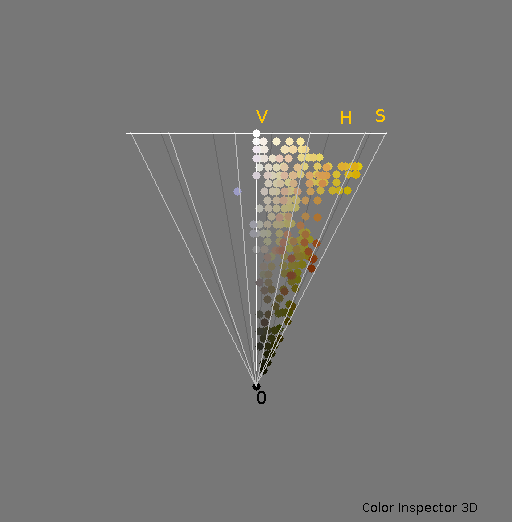
\includegraphics[width=4cm]{resultat/luminance1.png}
 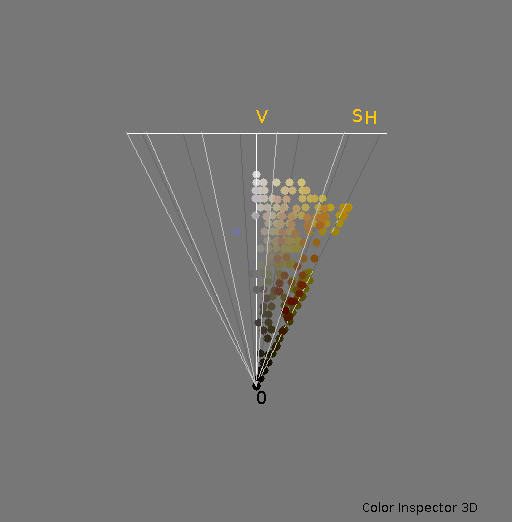
\includegraphics[width=4cm]{resultat/luminance2.png}
 \caption{Graphique de l'espace colorimétrique HSV des images \textit{it1\_72pp} et \textit{it1\_72pp\_sombre}}
 \end{center}
\end{figure}

On voit clairement que la plus grande valeur de luminance de l'image sombre est bien inférieure
à la valeur maximum de l'image plus claire. En effet, l'image qui est plus sombre ne possède pas de pixel dans le haut du cône HSV.\\

Nous allons maintenant essayer de transformer l'image la plus sombre en l'image originale. Pour cela,
nous allons simplement ajouter une valeur identique dans les trois canaux RGB. Etant donné que la valeur 255
représente le blanc, il est possible d'éclaircir l'image en rapprochant la valeur de chaque canal de la valeur 255.

\begin{figure}[!h]
	\begin{center}
	\begin{tabular}{|c|c|c|}
 		\hline
 		it1\_72pp & it2\_72pp & it3\_72pp\\
 		\hline
 		30 & 40 & 60\\
 		\hline
	\end{tabular}
	\caption{Valeur ajouté à l'image sombre pour obtenir l'image d'origine}
	\end{center}
\end{figure}

Lorsque nous effectuons la différence entre l'image originale et l'image transformée, nous observons le résultat suivant :

\begin{figure}[!h]
 \begin{center}
 \includegraphics[width=4cm]{resultat/difference_luminance.png}
 \caption{Résultat de la différence entre l'image original et l'image modifié}
 \end{center}
\end{figure}

Nous pouvons voir qu'il y a une différence sur les points verts foncés et les jaunes, car ceux-ci sont bleu sur la différence. Lorsque nous regardons la valeur de chaque canal pour ces points, on voit que les canaux rouge et vert ont la même valeur, tandis que le bleu est casiment null. Cela nous permet de faire ressortir le défaut de cette méthode qui est que la luminance n'utilise pas les mêmes coéfficiants pour chaque canaux. C'est pourquoi il exite des espaces colorimétriques particulier pour cette valeur. 

\section{Rétablissement de la saturation}
La saturation peut être définie comme étant la chromaticité de la couleur. Elle est l'intensité de la couleur, plus
la saturation est importante et plus la couleur paraît fade. Pour mettre en évidence cette saturation, nous analysons
l'espace colorimétrique HSV des images \textit{it2\_72pp} et \textit{it2\_72\_gris}, dont la première est plus saturée
que la seconde.\\

\begin{figure}[!h]
 \begin{center}
 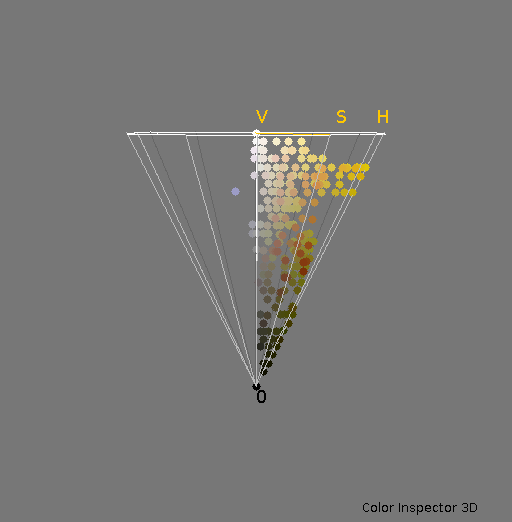
\includegraphics[width=4cm]{resultat/saturation1.png}
 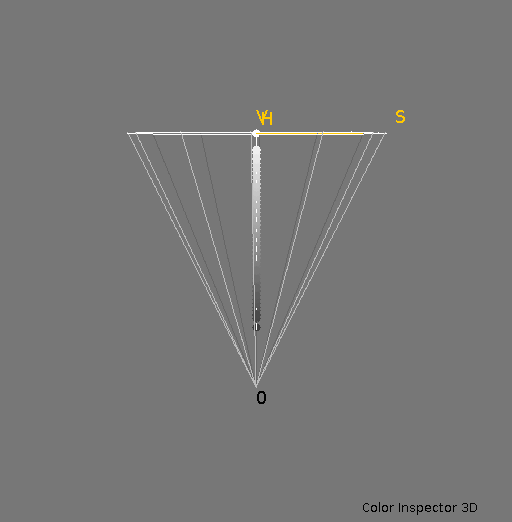
\includegraphics[width=4cm]{resultat/saturation2.png}
 \caption{Graphique de l'espace colorimétrique HSV des images \textit{it2\_72pp} et \textit{it2\_72\_gris}}
 \end{center}
\end{figure}

Sur ces images, l'information de saturation est représentée sur l'axe des x. On voit que sur l'image \textit{it2\_72\_gris} la
valeur de la saturation reste à 0, ce qui fait que l'ensemble des pixels restent au centre du cône. On voit qu'il n'est pas
possible de transformer l'image \textit{it2\_72\_gris} en l'image \textit{it2\_72pp}, car l'information \textit{value} n'est pas
connue et l'image ne changerait pas si on modifiait la saturation. C'est pourquoi nous utiliserons l'image \textit{it2\_72\_saturation\_faible}
pour nos tests sur le changement de la saturation. Voici dans un premier temps les graphiques des images dans le modèle HSB.

\begin{figure}[!h]
 \begin{center}
 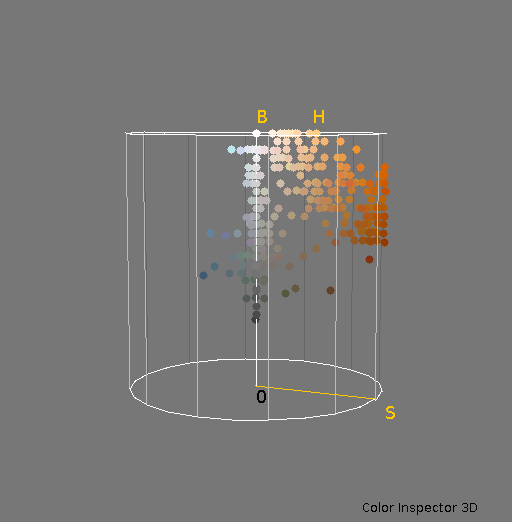
\includegraphics[width=4cm]{resultat/saturation1_2.png}
 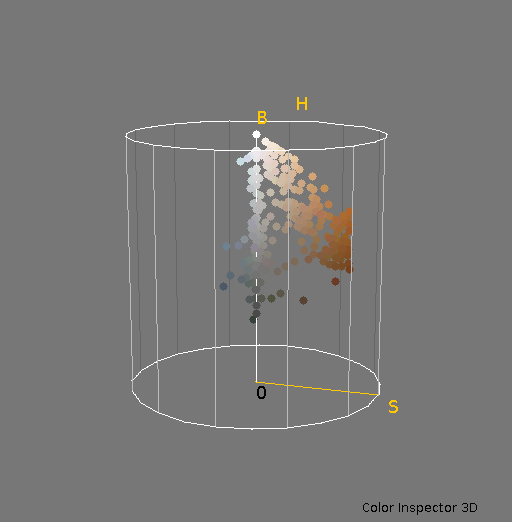
\includegraphics[width=4cm]{resultat/saturation2_2.png}
 \caption{Graphique de l'espace colorimétrique HSB des images \textit{it2\_72pp} et \textit{it2\_72\_saturation\_faible}}
 \end{center}
\end{figure}
\newpage

On voit avec ces graphiques que l'image \textit{it2\_72\_saturation\_faible} possède un \textit{value} différent de 0, donc si on 
multiplie la saturation par une valeur définie, il est possible de retrouver l'image \textit{it2\_72pp}. Cependant, on voit que 
la saturation n'est pas la seule valeur qui différencie les deux images, la luminance est également très différente. En multipliant
la saturation par 1,3 nous obtenons le résultat suivant :

\begin{figure}[!h]
 \begin{center}
 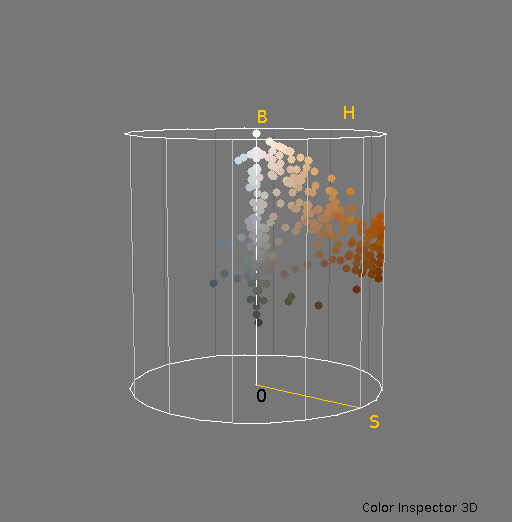
\includegraphics[width=4cm]{resultat/resultat_saturation.png}
 \caption{Résultat de la modification de la saturation}
 \end{center}
\end{figure}

\section{Transformation de la teinte}
La teinte est la forme la plus pure d'une couleur. Ce qui signifie qu'elle ne peut pas représenter le blanc, le noir ou le gris.
Pour modifier la couleur de l'image pour que le chiffre devienne vert, nous modifions la teinte en lui ajoutant la valeur 90.
Nous avons pris la valeur 90, car on peut voir sur le cercle de la teinte que le vert est à peu près à 90° de la couleur bleue.
Cela nous donne le résultat suivant : 
\begin{figure}[!h]
 \begin{center}
 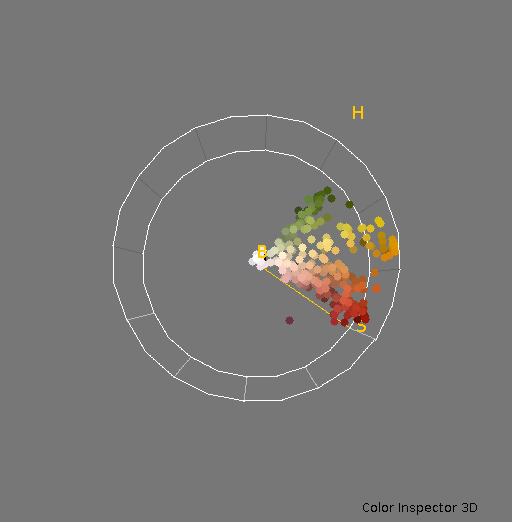
\includegraphics[width=4cm]{resultat/teinte1.png}
 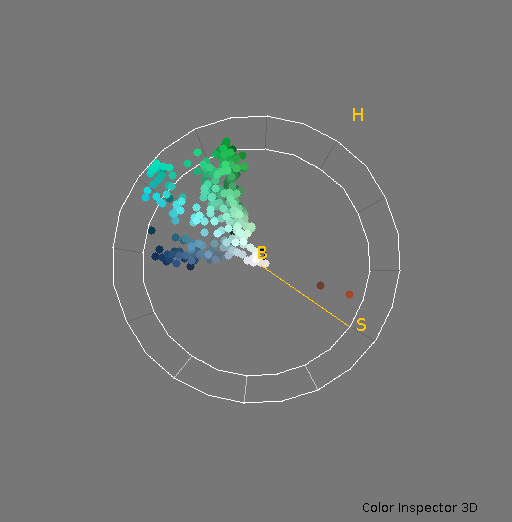
\includegraphics[width=4cm]{resultat/teinte2.png}
 \caption{Graphique de l'espace colorimétrique HSB de l'image \textit{it3\_72pp} et du résultat de la transformation}
 \end{center}
\end{figure}

\section{Analyse dans des espaces couleur adaptés}
Les personnes souffrant de daltonisme ont des difficultés à voir les formes dans les images que nous analysons. 
Voici dans un premier temps la représentation graphique des images \textit{it3\_72pp} et \textit{it3\_72\_sans\_5} que nous
allons analyser afin de comprendre les problèmes de ces personnes.
\begin{figure}[!h]
 \begin{center}
 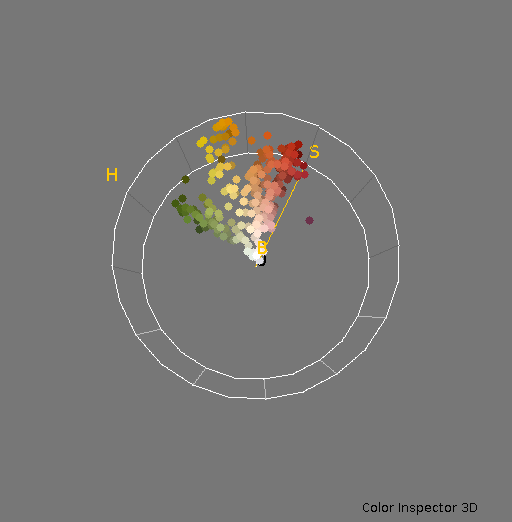
\includegraphics[width=4cm]{resultat/compare1_1.png}
 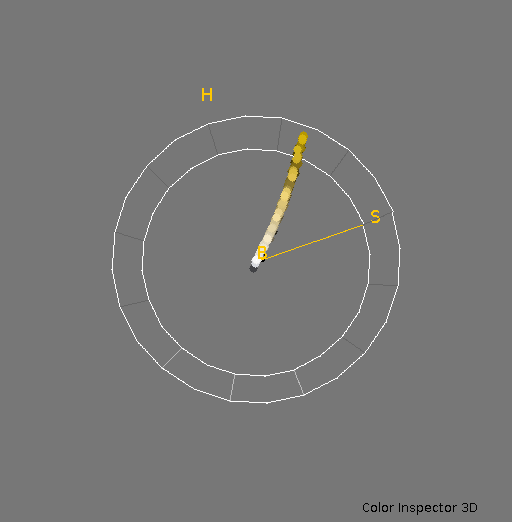
\includegraphics[width=4cm]{resultat/compare1_2.png}
 \caption{Graphique de l'espace colorimétrique HSB des images \textit{it3\_72pp} et \textit{it3\_72\_sans\_5}}
 \end{center}
\end{figure}

Sur ces images on peut considérer que l'image \textit{it3\_72pp} représente ce qui est visible par les personnes saines alors
que l'image \textit{it3\_72\_sans\_5} représente ce qui est visible par les personnes atteintes de daltonisme.
On peut voir sur ce premier résultat que certains types de daltonisme ne voient qu'un nombre infime de teintes. En effet, sur 
l'ensemble des teintes présentes dans l'image, une seule est visible par une personne malade.

\begin{figure}[!h]
 \begin{center}
 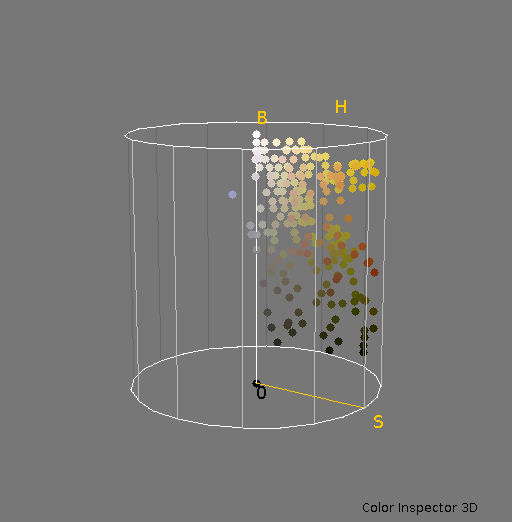
\includegraphics[width=4cm]{resultat/compare2_1.png}
 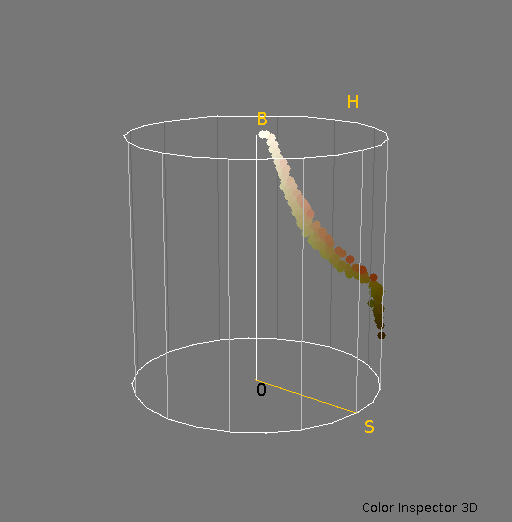
\includegraphics[width=4cm]{resultat/compare2_2.png}
 \caption{Graphique de l'espace colorimétrique HSB des images \textit{it1\_72pp} et \textit{it1\_72\_sans\_cercle}}
 \end{center}
\end{figure}

Sur ce second exemple, on voit que ce type de daltonisme ne perçoit que les couleurs dont la luminance est proportionnelle à 
la saturation.

\section{Conclusion}
Nous avons pu voir, lors de ce TP, différents modèles colorimétriques permettant de visualiser les informations de luminance, de 
teinte et de saturation. Bien que l'oeil humain soit composé de cônes pouvant percevoir de l'information dans le modèle
colorimétrique RGB, nous avons vu que les informations HSB avaient un impact important sur la vision de l'oeil humain.

\newpage

\section{Annexes}
\begin{lstlisting}[caption=Macros de modification de la luminance d'une image]
macro "augmentation_luminance" {

// recuperation du ID de l'image
image = getImageID();

valeur = getNumber ("quelle augmentation (absolue) de luminance",valeur);

if(valeur > 255) 
    valeur = 255;

Dialog.create("Debut");
Dialog.addMessage(" Cliquer sur OK pour commencer le traitement ");
Dialog.show();

setBatchMode(true);

// recuperation de la taille W x H du plan de fourier
W = getWidth();
H = getHeight();

run("Duplicate...", "title=luminance augmentee");
image_luminance_aug = getImageID();

// 
max_1 = 0; 
i_max_1 = 0;
j_max_1 = 0;

for (j=0; j<H; j++) {
   for (i=0; i<W; i++) 
	{
	selectImage (image);
	couleur_avant = getPixel(i,j);
	R_avant = (couleur_avant & 0xff0000) >> 16;
	G_avant = (couleur_avant & 0x00ff00) >> 8;
	B_avant = (couleur_avant & 0x0000ff) ;

	R_apres = R_avant + valeur;
	G_apres = G_avant + valeur;
	B_apres = B_avant + valeur;

	couleur_apres = ((R_apres & 0xff ) << 16) + ((G_apres & 0xff) << 8) + B_apres & 0xff;

	selectImage (image_luminance_aug);
	setPixel(i,j,couleur_apres);
	}
}

setBatchMode(false);

Dialog.create("Fin");
Dialog.addMessage(" Cliquer sur OK pour terminer le traitement");
Dialog.show();
}
\end{lstlisting}

\begin{lstlisting}[caption=Macros de modification de la saturation d'une image]
macro "augmentation_saturation" {

// recuperation du ID de l'image
image = getImageID();

valeur = getNumber ("quelle augmentation (absolue) de saturation",valeur);

if(valeur > 255) 
    valeur = 255;

Dialog.create("Debut");
Dialog.addMessage(" Cliquer sur OK pour commencer le traitement ");
Dialog.show();

setBatchMode(true);

// recuperation de la taille W x H du plan de fourier
W = getWidth();
H = getHeight();

//dusplication de l'image
run("Duplicate...", "title=saturation");
image_saturation_aug = getImageID();

//changement d'espace colorimetrique
run("Color Space Converter", "from=RGB to=HSB white=D65");

//split des canaux
run("Split Channels");

//traitement sur les image
selectWindow("saturation (HSB) (green)");
run("Multiply...", "value="+valeur);

//merge des canaux 
run("Merge Channels...", "red=[saturation (HSB) (red)] green=[saturation (HSB) (green)] blue=[saturation (HSB) (blue)] gray=*None* keep ignore");

//changement d'espace colorimetrique
run("Color Space Converter", "from=HSB to=RGB white=D65");

setBatchMode(false);

Dialog.create("Fin");
Dialog.addMessage(" Cliquer sur OK pour terminer le traitement");
Dialog.show();

}
\end{lstlisting}

\begin{lstlisting}[caption=Macros de modification de la teinte d'une image]
macro "augmentation_teinte" {

// recuperation du ID de l'image
image = getImageID();

Dialog.create("Debut");
Dialog.addMessage(" Cliquer sur OK pour commencer le traitement ");
Dialog.show();


setBatchMode(true);


// recuperation de la taille W x H du plan de fourier
W = getWidth();
H = getHeight();

//dusplication de l'image
run("Duplicate...", "title=saturation");
image_saturation_aug = getImageID();

//changement d'espace colorimetrique
run("Color Space Converter", "from=RGB to=HSB white=D65");

//split des canaux
run("Split Channels");

//traitement sur les image
selectWindow("saturation (HSB) (red)");
run("Add...", "value="+90);

//merge des canaux
run("Merge Channels...", "red=[saturation (HSB) (red)] green=[saturation (HSB) (green)] blue=[saturation (HSB) (blue)] gray=*None* keep ignore");

//changement d'espace colorimetrique
run("Color Space Converter", "from=HSB to=RGB white=D65");

setBatchMode(false);

Dialog.create("Fin");
Dialog.addMessage(" Cliquer sur OK pour terminer le traitement");
Dialog.show();
}
\end{lstlisting}

%TODO ajout de la teinte
\end{document}
